\documentclass[a4paper,10pt]{article}
\usepackage[utf8]{inputenc}
\usepackage[T1]{fontenc}
\usepackage{mathpazo}
\linespread{1.05}
\usepackage{amsmath}
\usepackage{helvet}
\renewcommand{\familydefault}{\sfdefault}
\usepackage{cite}		% para contraer referencias
\usepackage[spanish]{babel}
\usepackage{float}
\usepackage[letterpaper, margin=2.5cm]{geometry}
\usepackage{setspace}  
\usepackage{graphicx}
\usepackage{tikz}
\usepackage{tikz-uml} 
\usepackage{subfigure}
\usepackage{hyperref}
\usepackage{times}
\usepackage{color}
\usepackage{enumerate}
\definecolor{gray97}{gray}{.97}
\definecolor{gray75}{gray}{.75}
\definecolor{gray45}{gray}{.45}
\usepackage{listings}
\lstset{ frame=Ltb,
	framerule=0pt,
	aboveskip=0.5cm,
	framextopmargin=3pt,
	framexbottommargin=3pt,
	framexleftmargin=0.4cm,
	framesep=0pt,
	rulesep=.4pt,
	backgroundcolor=\color{gray97},
	rulesepcolor=\color{black},
	%
	stringstyle=\ttfamily,
	showstringspaces = false,
	basicstyle=\small\ttfamily,
	commentstyle=\color{gray45},
	keywordstyle=\bfseries,
	%
	numbers=left,
	numbersep=15pt,
	numberstyle=\tiny,
	numberfirstline = false,
	breaklines=true,
}

% minimizar fragmentado de listados
\lstnewenvironment{listing}[1][]
{\lstset{#1}\pagebreak[0]}{\pagebreak[0]}

\lstdefinestyle{consola}
{basicstyle=\scriptsize\bf\ttfamily,
	backgroundcolor=\color{gray75},
}

\usepackage{mathtools}
\DeclarePairedDelimiter{\ceil}{\lceil}{\rceil}
\DeclarePairedDelimiter{\floor}{\lfloor}{\rfloor}

\begin{document}
	
\begin{center}
	\LARGE\textbf{Universidad de Costa Rica}\\
	\textbf{Facultad de Ingeniería}\\
	\textbf{Escuela de Ciencias de la Computación e Informática}\\ \ \\ \ \\
	\Large 	Proyecto Integrador de Redes y Sistemas Operativos\\
	Grupo 3\\
	I Semestre 2023\\ \ \\
\end{center}


\begin{center}
	\huge\textbf{Armador de figuritas con piezas plásticas (Entrega 1)} \\ \ \\ \
\end{center}

\begin{center}
	\LARGE\textbf{Profesores:}\\
	Tracy Hernández\\ \
	Rafael Arroyo\\ \ \\ \ \\
	\LARGE\textbf{Estudiantes:}\\
	Joseph Núñez $|$ C05582 \\ \  
	Omar Camacho Calvo $|$ C11476 \\ \ 
	Oscar Fernández Jiménez $|$ C12840 \\ \ 
	Pablo Rodríguez Navarro $|$ B66060 \\ \ \\ \ \\
	%Si hay más integrantes se agregan
	\LARGE\textbf{15 de abril del 2023}
\end{center}
	
	\thispagestyle{empty}
	\newpage
	
	\tableofcontents
	\setcounter{secnumdepth}{1}
	\newpage
	
	\section{Introducción}
	%Se comienza a escribir la introducción
	El objetivo del proyecto es construir todo el entorno en cuanto a la funcionalidad cliente servidor se refiere. Para lograrlo se necesita ir construyendo los diversos componentes por etapas y para esto es necesario poner en práctica todos los conocimientos adquiridos en los cursos de Redes y Sistemas Operativos.
	El proyecto consiste básicamente en crear servidores de piezas plásticas (Lego), que permitan a los diversos clientes puedan realizar peticiones y obtener dichas piezas. Para esto se ve en la necesidad de construir servidores intermedios que permitan tener la información de los distintos servidores de piezas y que permitan redirigir al cliente al servidor correspondiente.
	
	
	\section{Objetivos}	
	\begin{itemize}
	    \item Crear un servidor de piezas plásticas (Lego) que permita recibir peticiones, enviar respuestas y mantener control de las piezas.
	    \item Construir un servidor intermedio que almacene las direcciones y puertos de los diversos servidores de piezas, reciba peticiones y respuestas y se encargue de redirigir a los clientes a los servidores correspondientes.
	    \item Concebir un cliente que sea capaz de enviar solicitudes y recibir respuestas hacia y desde los servidores intermedios y permita mostrar el resultado de las mismas.
	\end{itemize}

	 \newpage

	\section{Descripción}
	Para esta primera entrega del proyecto, se ha desarrollado un cliente que tiene la capacidad de realizar solicitudes a un servidor de piezas plásticas (Lego) utilizando el protocolo HTTPS y una conexión TCP cifrada con SSL para garantizar la seguridad de la información.
	Una vez que el cliente envía la solicitud, el servidor enviará una respuesta con los datos solicitados, en caso de estar disponibles, caso contrario devolverá un error de disponibilidad.
 
	Una vez el cliente recibe la respuesta utilizará una clase Parser para analizar y extraer la información requerida de la respuesta del servidor. Si la respuesta contiene la información necesaria, el cliente muestra una lista de piezas plásticas necesarias para construir la figura deseada.
 
	Cada servidor cuenta con una lista de figuras, a la cual debemos añadir una figura formada por piezas de plástico única que sea representativa y sirva para posteriores entregas, en formar parte del inventario del servidor de piezas. Para este caso se escogió el Tucán como animal representativo.
 
	Es importante destacar que el Tucán es solo una de las muchas piezas plásticas que podrán estar disponibles en los servidores de piezas para las siguientes etapas.

	\begin{figure}[h]
 	  \centering
 	  
\includegraphics[scale=.2]{toucan.jpg}
	 \end{figure} \\ \
    \newpage
    \vfill
	 Las piezas que lo componen:
	 \begin{itemize}
	 	\item 1 brick 2x2 blue
	 		\begin{figure}[H]
 	  		\centering
 	  		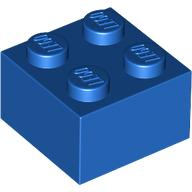
\includegraphics[scale=.2]{brick_2x2_blue.jpg}
		 	\end{figure}
		 	
		 \item 1 brick 1x2 blue
		 	\begin{figure}[H]
 		  	\centering
 		  	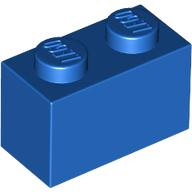
\includegraphics[scale=.2]{brick_1x2_blue.jpg}
		 	\end{figure} 
		 	
		 \item 2 brick 2x2 slope blue
                \begin{figure}[H]
 		  	\centering
 		  	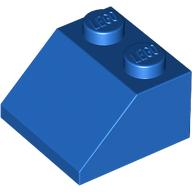
\includegraphics[scale=.2]{brick_2x2_slope_blue.jpg}
		 	\end{figure}
		 	
		 \item 1 brick 2x2 slope inverted blue
		 	\begin{figure}[H]
 		  	\centering
 		  	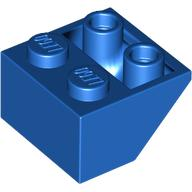
\includegraphics[scale=.2]{brick_2x2_slope_inverted_blue.jpg}
		 	\end{figure}
          
		 \item 1 brick 2x3 with arches red
		 	\begin{figure}[H]
 		  	\centering
 		  	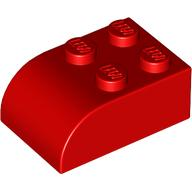
\includegraphics[scale=.2]{brick_2x3_with_arches_red.jpg}
		 	\end{figure}
    
		 \item 1 plate 2x3 yellow
		 	\begin{figure}[ht]
 		  	\centering
 		  	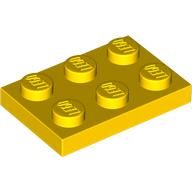
\includegraphics[scale=.2]{plate_2x3_yellow.jpg}
		 	\end{figure}
		 	
		 \item 2 brick 1x1 yellow eye
		 	\begin{figure}[ht]
 		  	\centering
 		  	
\includegraphics[scale=.2]{brick_1x1_yellow_eye.jpg}
		 	\end{figure}
	\end{itemize}
		 \newpage
          \vfill
	\section{Diseño}
    Se decidió implementar un paradigma de programación orientada a objeto en c++, para dicha implementación se crearon tres clases principales: IOManager, Parser y Socket; mismas que se detallan en los diagramas de a continuación:
    \vfill
    	 \begin{figure}[ht]
 	  \centering
 	  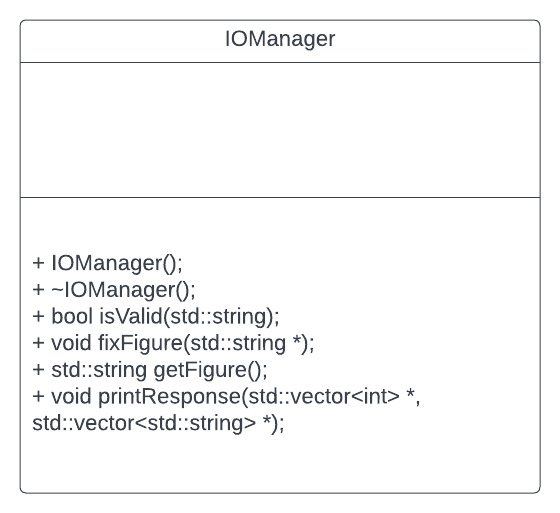
\includegraphics[scale=2]{IOManager.jpeg}
	 \end{figure}
	 
	 \begin{figure}[ht]
 	  \centering
 	  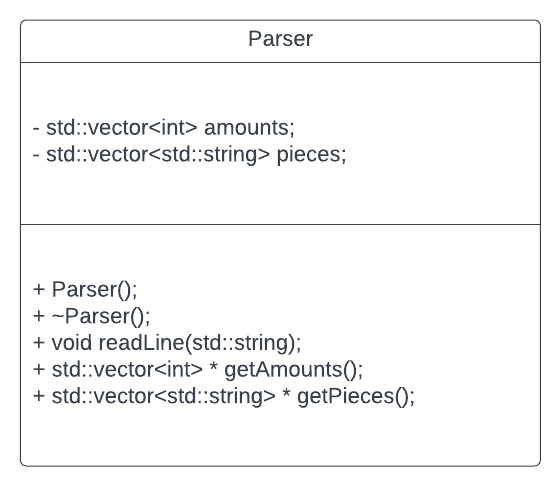
\includegraphics[scale=2]{Parser.jpeg}
	 \end{figure}

	 \begin{figure}[ht]
 	  \centering
 	  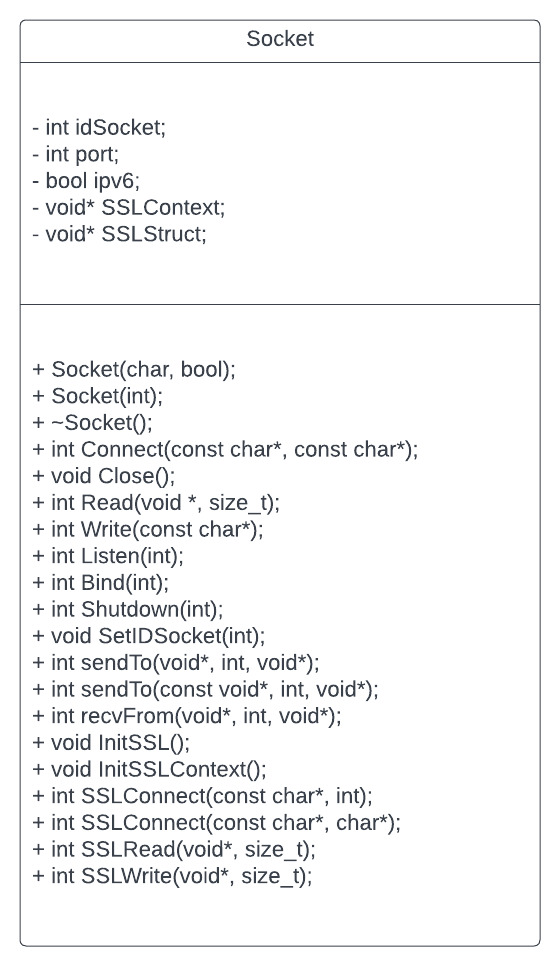
\includegraphics[scale=2]{Socket.jpeg}
	 \end{figure}
    \vfill
    \clearpage
	\newpage
	
	\section{Desarrollo}
	En primer lugar, se toma como base la clase Socket que se ha venido desarrollando a lo largo del curso, de la cual principalmente se hace del envío de mensajes TCP seguros mediante el protocolo Secure Sockets Layer (SSL). Esto se utiliza para establecer una conexión de red entre el dispositivo cliente y el server, esto se hace con el objetivo de transferir datos entre ellos, principalmente recibir la información de las piezas por parte del cliente.
 
	La clase Parser, por otro lado, se encarga de analizar la respuesta del servidor y extraer los datos relevantes (cantidad de piezas y piezas) para que puedan ser utilizados por la aplicación del cliente. Se espera que las respuestas del servidor estén en formato HTML, pues esta clase se encarga de determinar en qué parte del código HTML se encuentran tanto las piezas como la cantidad de las mismas, mediante una serie de expresiones regulares. La clase terminará guardando en una serie de estructuras todas las coincidencias halladas, para luego pasar dicha información a la siguiente clase.
 
	La tercera clase es la que interactúa directamente con el usuario de la aplicación. Esta clase se encarga de solicitar la información al usuario de la figura que desea consultar, y mostrar la respuesta del servidor de una manera más comprensible para el usuario. Al mostrar un listado de piezas junto a su cantidad.
	 También debe manejar errores de entrada y salida, como cuando el usuario ingresa una entrada inválida o cuando no se puede conectar al servidor.
 
	Finalmente, todas las clases anteriores se conectan mediante el archivo principal del programa, el cual se encarga montar la información necesaria para crear el socket, para luego enviar la información de la figura a la dirección de dicho socket.
 
	Una vez obtenida una respuesta, esta se lee en chunks de 1024 bytes, de los cuales se obtiene la información de cada línea de texto para posteriormente utilizar la clase Parser sobre dicha línea con el propósito de obtener los objetos esperado. Luego simplemente se llama la clase I/O para imprimir la información resultante en pantalla.

 	\subsection{Protocolo de comunicación}
	En esta sección nos encargaremos de describir previamente los aspectos relacionados al planteamiento del protocolo solicitado para mantener un intercambio de comunicación estable y consistente entre los dispositivos encargados de la solicitud y recepción de información

	Cabe destacar que para el funcionamiento del protocolo, cuando tenemos 3 tipos de host, los cuales son:
	Cliente: encargado de solicitar y recibir un HTML de la figura y poder pasear dicho html.
	Servidor intermediario: encargado de recibir la solicitud del cliente, seleccionar las mejores direcciones asociadas en su tabla de routing y responder/enviar solicitudes.
	Servidores de piezas: encargado de contener los HTML de dichas figuras y poder enviar/recibir paquetes con su informacion.
	
	Ahora bien, la función entidad principal de este protocolo se basa en la recepción y envío de señales o
	mensajes mediante el protocolo de transporte UDP por medio de un puerto en específico en cuando
	definimos como en 3141.
	Para esto, los primeros dispositivos que van a realizar su inicialización van a ser los servidores
	intermediarios, los cuales al levantarse comenzarían una escucha UDP por el puerto 3141, para quedar
	en espera a cargar su tabla de routing quedando lista para recibir valores, posterior a esto se levantarían
	los servidores de piezas y cargarían la lista de figuras internas que tenga cada 1, ya sea que tengan una
	figura propia o más de una, para por consiguiente, realizar un send to en UDP en el puerto 3141.
	
	Lo cual desembocaría en que esos servidores enviarán un paquete a ese puerto con un String que en
	formato [ip:figura:figura] y fuera recibido por cualquier dispositivo que se encontrara escuchando en el
	dicho puerto en Protocolo UDP,en donde, los primeros en recibir ese mensaje serían los receptores que están escuchando en ese mismo
	puerto (servidores intermedios).
	
	Con ese String enviado, los servidores intermediarios tendrían la capacidad de poder rellenar su tabla de
	routing, asociando en nombre de las figuras a su respectiva IP. Para posterior a esto, que en los
	servidores de piezas comenzarán a realizar una escucha por TCP por el mismo puerto para comenzar a
	atender solicitudes provenientes del servidor intermediario por parte del cliente.
	Ahora bien, al momento en que un host realice una conexión en necesidad de una figura del servidor de
	piezas, esta solicitud se dará enviada por https a los servidores intermedios concatenando el query
	string de la ip del servidor intermedio al nombre de la figura solicitada.
	Al ser el request recibido por el servidor intermedio, este procederá a buscar en su lista de routing el
	nombre de la figura y la lista de número de IP asociado a dicha figura, amén de encontrar la IP próxima, y
	poder enviar por TCP un paquete con un String que contendrá el nombre la figura al servidor de piezas
	respectivo, y que este servidor de piezas pueda responder con un response que contenga un string con
	el página en HTML de la figura solicitada, dicho HTML será recibido por el servidor intermedio y este sin
	ninguna modificación se enviara al cliente en su response de https y que éste, por medio de su aplicación
	cliente.cpp será capaz de parsear dicho HTML y poder ver la figura recibida

	\newpage
	
	\section{Manual de usuario}
	
    % Paso a paso de lo que espera el programa a la hora de ejecutarlo por ejemplo, si pide entradas.
	
	\subsection{Requerimientos de Software}
	%Que se ocupa para ejecutar el programa
	\begin{itemize}
		\item \textbf{Sistema Operativo: Ubuntu}
		\item \textbf{Arquitectura: x86 / x64 } 
	\end{itemize}
	
	\subsection{Compilación}
    %Paso a paso de como compilar el programa y ejecutarlo, acontinuación hay unos ejemplos
	\begin{listing}[style=consola, numbers=none]
	$ make$
	\end{listing}
	\begin{listing}[style=consola, numbers=none]
	$ cd bin$
	\end{listing}
	\begin{listing}[style=consola, numbers=none]
	$ ./Primera_Entrega$
	\end{listing}
	
	
	\subsection{Especificación de las funciones del programa}
    %Se específica lo que se espera que haga el programa, explicar de esto que funciona y que no funciona.
    Una vez compilado el programa e iniciada su ejecucción, se espera que el programa muestre un texto donde se le solicite al usuario el nombre de la figura a consultar, el mismo queda a la espera de la entrada; una vez se ingresa el dato, se procede a realizar la solicitud al servidor y dependiendo la respuesta, se muestra el resultado correspondiente.
    Si la figura existe, se debe mostrar la cantidad de piezas diferentes, la lista detalla de las piezas con cantidad y nombre y finalmente la cantidad total de piezas necesarias para armar la figura.

	
	\newpage
	
	\section{Casos de Prueba}
	Ejecución del programa
		\begin{figure}[ht]
 	  	\centering
 	  	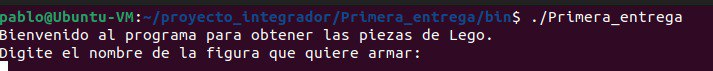
\includegraphics[scale=.5]{execution.jpeg}
	 	\end{figure}

	\noindent \textbf{Prueba 1: Solicitud completada correctamente}\\
	
		\begin{figure}[ht]
 	  	\centering
 	  	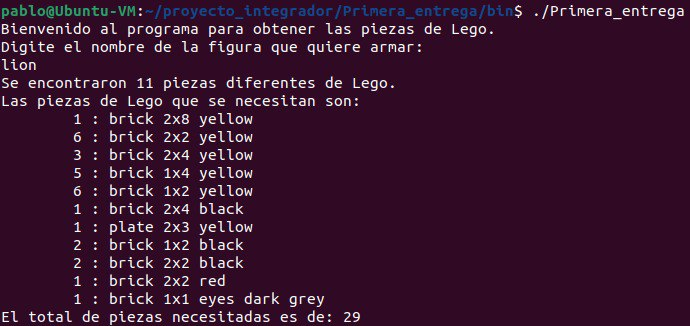
\includegraphics[scale=.5]{success.jpeg}
	 	\end{figure}
	
	\noindent \textbf{Prueba 2: Figura inexistente}\\
		\begin{figure}[ht]
 	  	\centering
 	  	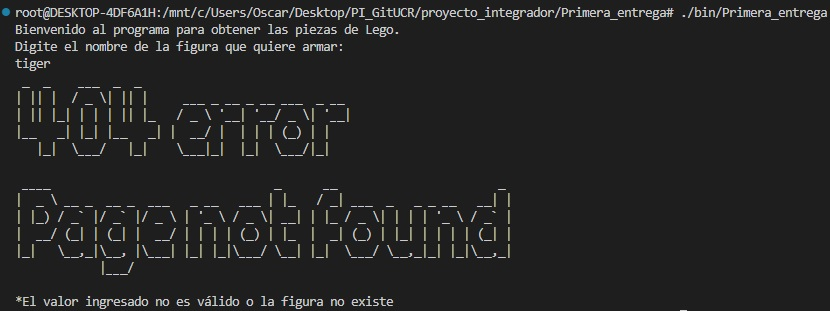
\includegraphics[scale=.7]{not_exist_animal.jpeg}
	 	\end{figure}
        \newpage
        \vfill
    	\noindent \textbf{Prueba 3: Entrada con números}\\%agregar las pruebas necesarias
    		\begin{figure}[ht]
 	  	\centering
 	  	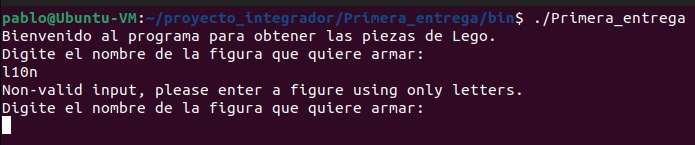
\includegraphics[scale=.5]{error_numbers.jpeg}
	 	\end{figure}
	 	
	 \noindent \textbf{Prueba 4: Palabras sin sentido}\\
		\begin{figure}[ht]
 	  	\centering
 	  	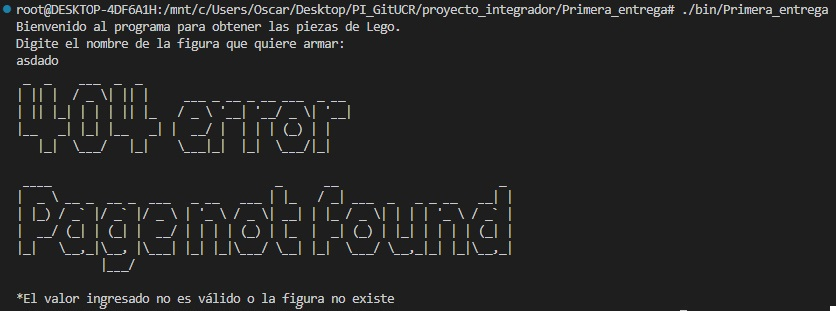
\includegraphics[scale=.7]{non_sense.jpeg}
	 	\end{figure}
    \vfill
    \clearpage
	
	
\end{document}


%Así se agrega una imagen
% \begin{figure}[h]
 %  \centering
 %  \includegraphics[scale=.2]{NombreDeImagen}
% \end{figure}
